\documentclass[11pt]{report}

\usepackage{MarioLeoYunStyle}

\usepackage{tikz}
\usepackage{float}

\title{\titleinfo}
\author{\authorinfo}
\date{}

\begin{document}

\maketitle
\thispagestyle{empty} % Removes the page number on the title page

\tableofcontents

\chapter{Introduction and Motivation}
\section{Introduction to the Problem}
Meshes and points are the most common 3D scene representations. However, although easily parallelizable, they are not differentiable. This limitation poses significant challenges for tasks that require gradient-based optimization, such as neural rendering and scene reconstruction.

\section{Background and Related Work}
Traditional scene reconstruction and rendering techniques have relied heavily on mesh-based representations. While effective, these methods often struggle with complex scenes and require extensive manual effort to achieve high-quality results.

Neural rendering and radiance fields have emerged as powerful alternatives, leveraging neural networks to model the appearance and geometry of 3D scenes. These methods have demonstrated impressive results in generating photorealistic images and enabling novel view synthesis.

Point-based rendering and radiance fields offer another promising approach, combining the simplicity of point clouds with the flexibility of neural networks. This hybrid method aims to overcome the limitations of traditional mesh-based techniques while maintaining the benefits of differentiability and scalability.

\section{Overview of the Idea}
Prior research on the novel technique, 3D-Gaussian Splatting, presents the idea of representation of a scene using 3D Gaussians (Splats) [Kerbl et al., 2023]. 3D Gaussians are instantiated in a scene using Source From Motion (SFM) techniques. The properties of the 3D Gaussians are subsequently optimized using gradient descent. One limitation of this approach is the lack of control over the density of the Splats in the scene. This causes the results of the optimization process to be highly dependent on the quality of the point cloud output by the SFM process. For example, in areas that have been under-reconstructed or over-reconstructed, the density of the point cloud used to initialized from the source images will be too low or high, respectively, at those regions, causing the density of the Splats initialized accordingly to similarly be inappropriate for the representation of the scene.

To improve performance, Kerbl et al. presents the idea of Adaptive Density Control (ADC). At fixed intervals, the algorithm performs 3 operations: \textbf{Cloning}, \textbf{Splitting}, and \textbf{Pruning}. Each of these operations affects the density of the Splats in the scene, allowing the model to dynamically adjust the number of Gaussians, increasing the Splat density in under-reconstructed regions of the scene, and vice versa. Hence, the ADC process improves the representation of the scene over time and ensures that the Gaussians are distributed more effectively, focusing computational resources on the most important areas of the scene.

%, will first delete the Gaussians whose transparency $\alpha$ is less than a threshold $\epsilon_\alpha$.\\

%Then, it will add new Gaussians to the scene based on the density of the existing ones. This adaptive approach allows the model to dynamically adjust the number of Gaussians, improving the representation of the scene over time. The process ensures that the Gaussians are distributed more effectively, focusing computational resources on the most important areas of the scene.

\chapter{Implementation}

\section{Original Algorithm}
In this section, we describe the baseline architecture used as the foundation for our algorithm. The baseline is based on the 3D Gaussian Splatting (3D-GS) technique, which models a scene using 3D Gaussians. The original paper presents a method for real-time radiance field rendering using a fixed number of Gaussians. Figures from the original paper are reproduced here to illustrate the baseline architecture.

Firstly, we initialize our initial scene representation using the point cloud generated by the SFM process on a set of input images. We also obtain and store the camera position of each input image from the SFM process.

At every iteration, we select one of the camera positions, and render the scene using that camera position. The rendered image is then compared with the corresponding input image, and a loss value is calculated. Gradients from the loss are then backpropogated to the parameters of the Splats, and used for their optimization.

At fixed intervals in the optimization process, we also carry out Adaptive Density Control, which comprises the following 3 operations: \textbf{Cloning}, \textbf{Splitting}, and \textbf{Pruning}. Notably, the ADC is called after the gradients have been back-propogated from the loss value, but before the parameters of the Splats in the model are stepped according to their gradients.

\begin{center}
\begin{minipage}{0.6\linewidth}
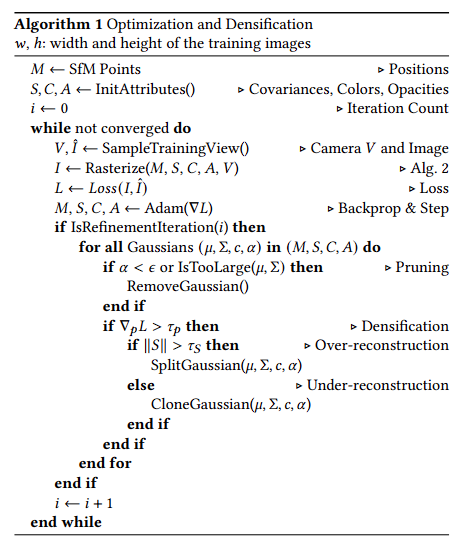
\includegraphics[width = \linewidth]{assets/original_optimization_and_densification}
\captionof{figure}{Summary of optimization and densification algorithms [Kerbl et al., 2023].}
\end{minipage}
\end{center}

\subsection{Cloning}
The Clone operation selects and replicates a subset of Splats in the model. Eligible Splats are selected using a gradient threshold; Splats with a positional gradient exceeding the gradient threshold, and also occur in under-reconstructed regions of the scene (determined by comparing the Splat's scale against the density of the scene), are selected to be Cloned. For each selected Splat, an exact copy is made, including all of its parameters, such as position, scaling, rotation, color, and transparency. Importantly, the gradients of the original Splats' attributes are not copied to the new Splat. Subsequently, during the optimization step, the original Splat has its attributes stepped according to their gradients, while the newly Cloned Splat remains unchanged.

\subsection{Splitting}
The Split operation selects and splits a subset of Splats in the model. Similarly, eligible splats are selected for splitting by comparing their gradients against a threshold, as well as their scaling against the scene density. Each selected Splat is split into 2 copies, each with their scale divided by a factor of $\phi = 1.6$. To determine the positions of the 2 newly instantiated Splats, the original 3D Gaussian is used as a probability density function for sampling.

\subsection{Pruning}
The Prune operation selects and removes a subset of Splats from the model, by comparing their transparency values, $\alpha$, against a minimum acceptable transparency, $\epsilon_{\alpha}$. Any splats in the scene with $\alpha < \epsilon_{\alpha}$ are removed from the representation, and are not rendered as part of the output image.

\section{Algorithm Improvements}
One issue with the implementation of the ADC is that the operations are heuristic in nature, and may hence be sub-optimal, because they are non-differentiable and may misalign with the final training obective [Zhan and Liang et al., 2024]. Zhan and Liang et al. instead proposes the technique of Evolutive Primitive Organization, which builds upon the original implementation of ADC by introducing optimizable parameters, used in the Cloning and Splitting operations that allow them to be optimized using the backpropogation of gradients from the loss to the parameters. Our project aims to build upon these ideas and methodologies.

\subsection{Cloning}
We aim to optimize the position of the newly Cloned Splat, which is a product of its growth direction $d$, as well as growth length $l$, relative to the original Splat which it was Cloned from (its Parent). We denote the position of the original Splat $\mu$, and the relative position of the newly Cloned Splat $\Delta \mu$, such that $\Delta \mu = dl$.

To this extent, we introduce 2 new learnable parameters for each Splat: \textbf{growth direction probabilities} ($p$), and \textbf{growth length s} ($s$), which will be used in the calculation of $d$ and $l$ respectively.

% \begin{center}  
% \begin{minipage}{0.4\linewidth}
% 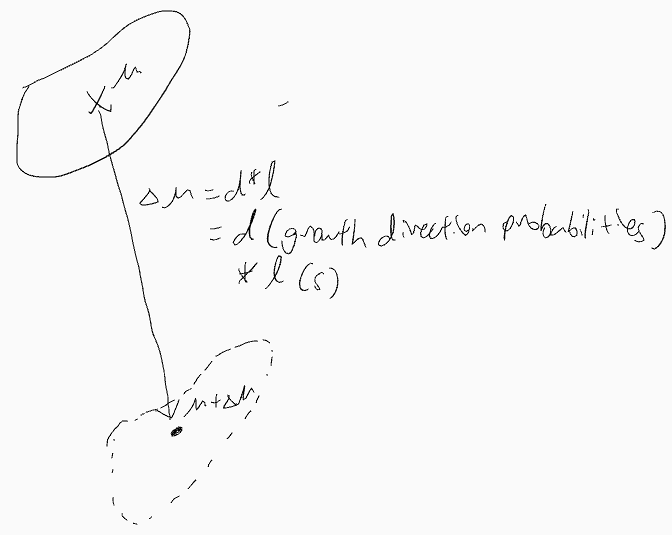
\includegraphics[width = \linewidth]{assets/clone}
% \captionof{figure}{Position of newly Cloned Splat.}
% \end{minipage}
% \end{center}
\begin{figure}[H]
    \centering
    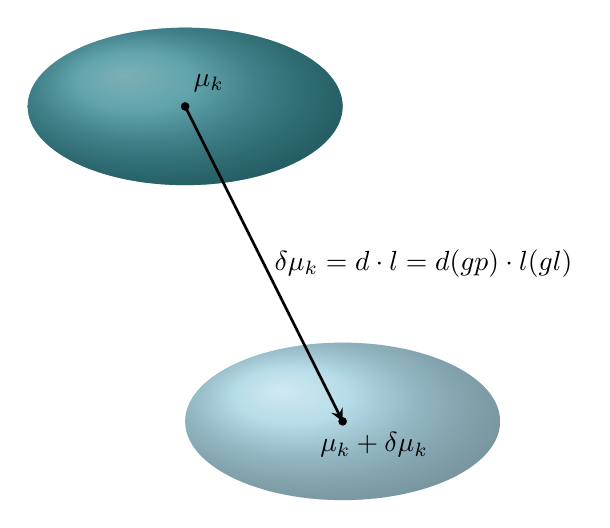
\begin{tikzpicture}
    \def\x{0}
    \def\y{2}
    \def\xf{2}
    \def\yf{-2}
    \def\sx{2}
    \def\sy{1}
    % Draw the larger ellipse labeled X_μ
    % \draw[thick] (\x, \y) ellipse ({\sx} and {\sy});
    \def\dx{1}
    \def\dy{1}
    % \def\s{1.5}
    \def\gop{0.5}
    \definecolor{dark_cyan}{RGB}{5, 104, 110}
    \definecolor{light_cyan}{RGB}{173, 216, 230}
    
    \fill[dark_cyan] (\x, \y) ellipse ({\sx} and {\sy});
    \shade[ball color=light_cyan, opacity=\gop] (\x, \y) ellipse ({\sx} and {\sy});
    \fill (\x, \y) circle (1.5pt); % Point at the center of X_μ
    \node at (\x + 0.3, \y + 0.3) {\textbf{$\mu_k$}};
    
    % Draw the smaller dashed ellipse labeled "interior"
    \fill[light_cyan] (\xf, \yf) ellipse ({\sx} and {\sy});
    \shade[ball color=light_cyan, opacity=\gop] (\xf, \yf) ellipse ({\sx} and {\sy});
    \fill (\xf, \yf) circle (1.5pt); % Point at the center of interior
    % \node[below] at (0, -2.5) {\textit{interior}};
    
    % Draw points and arrow
    \fill (\x, \y) circle (1.5pt); % Point at the center of X_μ
    \fill (\xf, \yf) circle (1.5pt); % Point at the center of interior
    \draw[thick, ->, >=stealth, line width=1pt] (\x, \y) -- (\xf, \yf) node[midway, right] {$\delta \mu_k = d \cdot l = d (gp) \cdot l(gl)$};
    % \draw[thick, ->, >=stealth, line width=2.5pt] ({\xf + (\x - \xf) * 0.000001}, {\yf + (\y - \yf) * 0.000001}) -- (\xf, \yf);
    
    \node at (\xf+0.4, \yf - 0.3) {\textbf{$\mu_k + \delta \mu_k$}};
    % Annotate components of the formula
    % \node[right] at (\xf, \yf + 1) {$d$ (growth direction probabilities)};
    % \node[right] at (\xf, \yf + 0.5) {$l(s)$};
\end{tikzpicture}
    \caption{Your caption here}
    \label{fig:your_label}
\end{figure}

\subsection{Splitting}
We aim to optimize the relative positions of the 2 newly split Splats. We denote the position of the original Splat $\mu$, and the relative positions of the 2 newly split Splats $\Delta \mu$ and $- \Delta \mu$. $\Delta \mu$ is optimized through the introduction of a learnable parameter \textbf{s prime} ($s'$), which is used in the calculation of $\Delta \mu$

We also aim to optimize the scale $\varphi$, of the 2 newly split Splats with respect to their Parent. We introduce the variable $\phi$, which is used as a scaling factor such that $\varphi_{new} = \frac{\varphi_{old}}{\phi}$. $\phi$ is optimized through the introduction of another learnable parameter \textbf{v} ($v$), which is used in its calculation.

\begin{center}
\begin{minipage}{0.4\linewidth}
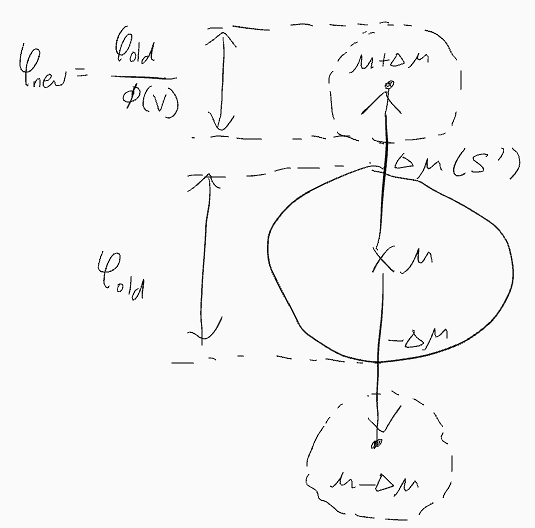
\includegraphics[width = \linewidth]{assets/split}
\captionof{figure}{Position and scale of newly split Splats.}
\end{minipage}
\end{center}

\subsection{Pruning}
We did not work on modifying the original implementation of the Prune operation, choosing instead to focus on the Clone and Split operations. However, we believe that our methodology can be extended to apply to the Prune operation in future work, because it similarly decides the subset of Splats to remove from the model in a heuristic manner. In particular, the minimum threshold for the transparency of the Splats, $\epsilon_{\alpha}$ is selected heuristically. In an improved implementation, we could also implement $\epsilon_{\alpha}$ as an optimizable parameter, allowing the Pruning operation to be optimizable using gradient descent from training objectives.

%To improve upon the baseline, we implemented several enhancements. The key improvement is the introduction of Adaptive Density Control, which dynamically adjusts the number of Gaussians in the scene. Every 100 iterations, Gaussians with transparency $\alpha$ below a threshold $\epsilon_\alpha$ are removed, and new Gaussians are added based on the density of existing ones. This adaptive approach ensures a more efficient and accurate representation of the scene. Figures are included to explain the idea and logic behind these improvements.

\section{Implementation Details}
%TODO: add code assets
The improvements were implemented in Python, using the PyTorch framework. The enhanced ADC mechanism was integrated into the training loop, allowing for dynamic adjustment of Gaussians during training.

\subsection{Cloning}
\subsubsection{Forward Pass}
Zhan and Liang et al. provided pseudocode for the implementation of a suitable algorithm. In this algorithm, we choose to optimize either the growth direction $d$, or the growth length $l$. Firstly, the chosen parameter is discretized, with a set of uniformly distributed possible values for the parameter created. Each Splat is then assigned a learnable set of probabilities, with each probability representing the probability that the corresponding value for the parameter is selected. In the forward pass, the Argmax function is used to select the value for the parameter with the highest probability, which is used for the calculation of $\Delta \mu$. However, the Argmax function disrupts the flow of gradients from the loss to the input parameters (in this case the set of probabilities). Instead, the algorithm propogates gradients as though the Softmax function had been used instead. This allows for effective optimization of the set of probabilities according to training objectives.
\begin{center}
\begin{minipage}{0.6\linewidth}
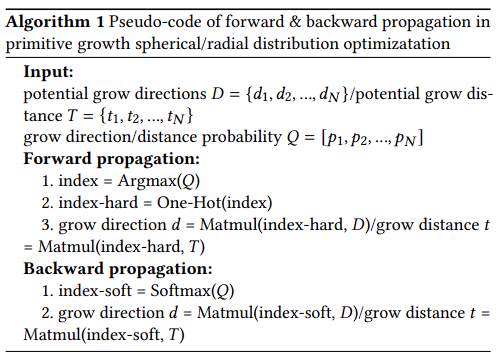
\includegraphics[width = \linewidth]{assets/clone_algo}
\captionof{figure}{Pseudocode of algorithm for learnable Cloning of Splats [Zhan and Liang et al.].}
\end{minipage}
\end{center}
In their implementation, Zhan and Liang et al. chose to optimize $d$ using the aforementioned algorithm. For $l$, they instead chose to directly learn the growth distance by using the standard deviation of the Parent Splat as a constraint. More specifically, they set $l = v \times \frac{1}{1 + e^{-s}}$, where $s$ is a learnable parameter and $v = 2 \times \sigma$, where $\sigma$ is the maximum standard deviation of the Parent Splat.

Our project reimplements the work of Zhan and Liang et al., similarly choosing to optimize Clone direction $d$ using the algorithm shown in \textbf{Figure 2.4}, by learning the parameter \textbf{growth direction probabilities} ($p$), and optimize Clone length $l$ using the formula $l = v \times \frac{1}{1 + e^{-s}}$, by learning the parameter \textbf{growth length s} ($s$).

We employ the reparameterization trick in our forward pass, detaching appropriate tensors from the computation graph such that the actual growth direction $d$ is selected using the Argmax function, but the calculation of gradients in the backward pass is performed as though the Softmax function was used instead.

\subsubsection{Backward Pass}
In the backward pass of the original 3D-GS implementation by Kerbl et al., the backward pass of the image rendering process calculates gradients for the original parameters of the Splats, which include their positions $\mu$. Unfortunately, the computation of gradients in the backward pass do not flow further down the computation graph to our newly introduced learnable parameters $p$ and $s$.

Hence, we manually calculate and propogate the gradients of $p$ and $s$ using chain rule. We know that for the Clone operation, the formula is as follows:
\[ \mu_{new} = \mu_{old} + \Delta \mu  \]
\[ = d(p) \times l(s) \]
We also know that the parameters $p$ and $s$ affect no other parameters in the model, and hence their impact on the loss value is dependent solely on their impact on $\mu_{new}$. Hence, we can say that
\[ \frac{\delta loss}{\delta p} = \frac{\delta loss}{\delta \mu_{new}} \times \frac{\delta \mu_{new}}{\delta p} \]
and similarly
\[ \frac{\delta loss}{\delta s} = \frac{\delta loss}{\delta \mu_{new}} \times \frac{\delta \mu_{new}}{\delta s} \]

Note that $\frac{\delta loss}{\delta \mu_{new}}$ can be obtained from the back-propogation of gradients from the loss to the means of the Splats, which is calculated in the original implementation by Kerbl et al.. To obtain the gradients for only the newly Cloned Splats, we store a mask of the newly Cloned points, when they are created.

To obtain $\frac{\delta \mu_{new}}{\delta p}$ and $\frac{\delta \mu_{new}}{\delta s}$, we can use PyTorch's automatic gradient calculation to automatically calculate them using the positions of the newly Cloned Splats, when they are calculated.

In actual implementation, we note that since $\frac{\delta loss}{\delta \mu}$ is a $N \times 3$ matrix, where $N$ is the total number of Splats, with $\frac{\delta loss}{\delta \mu}_{ij}$ representing the contribution to the loss from the $a$-coordinate of $\mu_{i}$, with
\[ a = \begin{cases}
x & \textrm{if }j=1\\
y & \textrm{if }j=2\\
z & \textrm{if }j=3\\
\end{cases} \]

we have to split $\frac{\delta \mu_{new}}{\delta p}$ into a $N \times 3 \times m$ tensor, where $m$ represents the number of discrete growth directions, with $\frac{\delta \mu_{new}}{\delta p}_{ijk}$ representing the contribution to the $a$-coordinate in $\mu_{new}$, by the probability of the $k$-th probability in $p_{i}$. The final multiplication hence gives us the desired shape $N \times m$, with each $\frac{\delta loss}{\delta p}_{ik}$ representing the contribution to the loss by the $k$-th probability in $p_{i}$.

Similarly, we split $\frac{\delta \mu_{new}}{\delta s}$ into a $N \times 3$ tensor, with $\frac{\delta \mu_{new}}{\delta s}_{ij}$ representing the contribution to the $a$-coordinate in $\mu_{new}$ by $s_{i}$. The final calculation of $\frac{\delta loss}{\delta s}$ hence gives the desired shape $N \times 1$.

It is important to note that we made the choice to update gradients for the Parent Splats, and not the newly Cloned Splats, because the effect on the loss calculated was due to the clone operation called using the Parent Splats' parameters.

\subsection{Splitting}
\subsubsection{Forward Pass}
The implementation of the Split operation by Zhan and Liang et al. optimizes the split mean shift, $\Delta \mu$, as well as the scaling factor of newly Split Splats, $\phi$.

For the optimization of $\Delta \mu$, each Splat in the scene is initialized with a learnable parameter $s'$. The formula $\Delta \mu = R(\sigma_{k} \times \frac{1}{1 + e^{-s'}})$ is then applied to calculate $\Delta \mu$, where $\sigma_{k}$ and $R$ are the standard deviation and rotation matrix of the Parent Splat. Once $\Delta \mu$ is calculated, the positions of the 2 newly Split Splats are initialized at $\mu + \Delta \mu$ and $\mu - \Delta \mu$ respectively.

For the optimization of $\phi$, each Splat is initialized with another learnable parameter $v$. The scaling factor $\phi$ is then calculated using the formula $\phi = 1.2 \times \frac{1}{1 + e^{-v}}$. Once $\phi$ is calculated, it is used to calculate the scale $\varphi$ of the newly Split Splats, using the formula $\varphi_{new1} =  \varphi_{new2} = \frac{\varphi_{old}}{\phi}$.

\subsubsection{Backward Pass}
To obtain the gradients for $s'$, we again note that the impact of $s'$ on the rendered image, and hence the loss, is limited to its impact on the positions of the newly Split Splats. Thus, we can again use the chain rule to calculate its gradient:
\[ \frac{\delta loss}{\delta s'} = \frac{\delta loss}{\delta \mu_{new}} \times \frac{\delta \mu_{new}}{\delta s'} \]

The impact of $v$ on the loss is limited to its impact on the scaling of the newly Split Splats.
\[ \frac{\delta loss}{\delta v} = \frac{\delta loss}{\delta \varphi_{new}} \times \frac{\delta \varphi_{new}}{\delta s'} \]

Similarly, $\frac{\delta loss}{\delta \mu_{new}}$ and $\frac{\delta loss}{\delta \varphi_{new}}$ are obtained from the back-propogation of gradients in the original 3D-GS implementation by Kerbl et al., and $\frac{\delta \mu_{new}}{\delta s'}$ and $\frac{\delta \varphi_{new}}{\delta s'}$ are obtained from invoking Pytorch's backward pass when $\mu_{new}$ and $\varphi_{new}$ are calculated respectively.

Importantly, $\varphi$ is also a $N \times 3$ tensor, representing the scaling of each Splat in each of its principal axes. Hence, the same logic is applied here to calculate $\frac{\delta \varphi_{new}}{\delta s'}$ as a $N \times 3$ tensor, with each $\frac{\delta \varphi_{new}}{\delta s'}_{ij}$ representing the contribution of $s'_{i}$ to the scaling of $\varphi_{new}$ in the axis corresponding to $j$.

For the Split operation, we update the gradients of the parameters of the newly Split Splats, since the Parent Splat is removed from the model entirely.

\chapter{Evaluation}

\section{Datasets}
We used the well-known Mip-NeRF360 dataset [Mildenhall et al. 2019] and LLFF dataset [Knapitsch et al. 2017] for training and testing our model. Additionally, we created two scenes for our own dataset and used synthetic scenes from the Synthetic Blender dataset. The datasets were preprocessed to extract training and testing images, which were then fed into the model for training and evaluation.

MipNeRF360 outdoor:
\begin{itemize}
    \item Bicycle 
    \item Stump
\end{itemize}

MipNeRF360 Indoor:
\begin{itemize}
    \item Counter (indoor)
\end{itemize}

Deep Blending:
\begin{itemize}
    \item Playroom
\end{itemize}

Tanks and Temples:
\begin{itemize}
    \item Truck
    \item Train
\end{itemize}

LLFF:
\begin{itemize}
    \item Horns (62 images)
    \item T-rex (55 images)
\end{itemize}

Same as NeRF, 3D-GS and the ERM, we take each 8th image for the test set and others for the training set.

\section{Training and Testing Results}
[Explain the training and testing results with graphs and elaborating on why they make sense, what could be improved.]

\section{Qualitative Results}
We test our model on both real-world scenes from previously published datasets, including the Mip-NeRF360 dataset, LLFF dataset, and synthetic scenes from the Deep Blending dataset. The specific scenes used from each dataset are as follows: 

For the MipNeRF360 outdoor dataset, we used the Bicycle and Stump scenes. From the MipNeRF360 indoor dataset, we used the Counter scene. For the Deep Blending dataset, we used the Playroom scene. From the Tanks and Temples dataset, we used the Truck and Train scenes. Lastly, from the LLFF dataset, we used the Horns scene with 62 images and the T-rex scene with 55 images.

[Big picture of as Figure 5 in 3DGS]



    \begin{tabular}{ccc}
        \textbf{Ground Truth} & \textbf{3D-GS} & \textbf{Ours} \\ \hline
            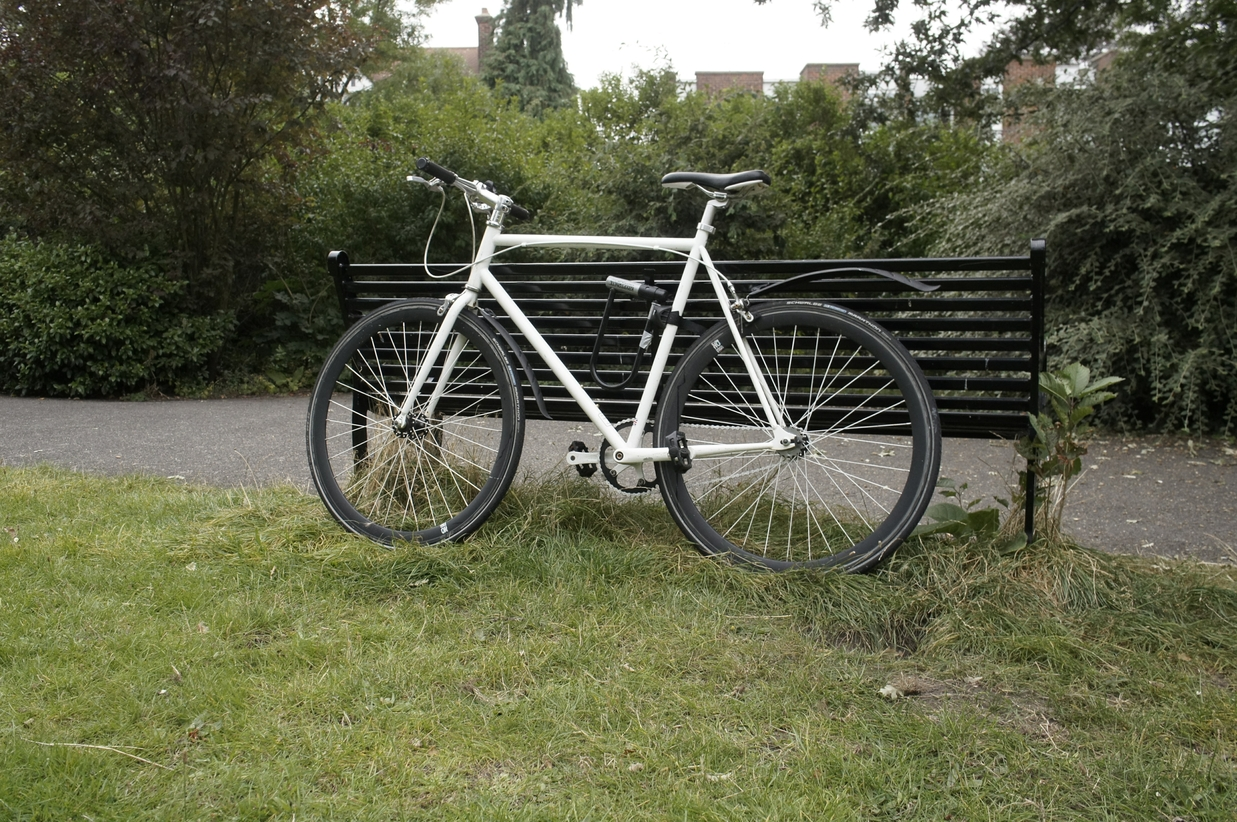
\includegraphics[width=0.3\textwidth]{../o-3dgs/eval/bicycle/test/ours_30000/gt/00000.png} &
            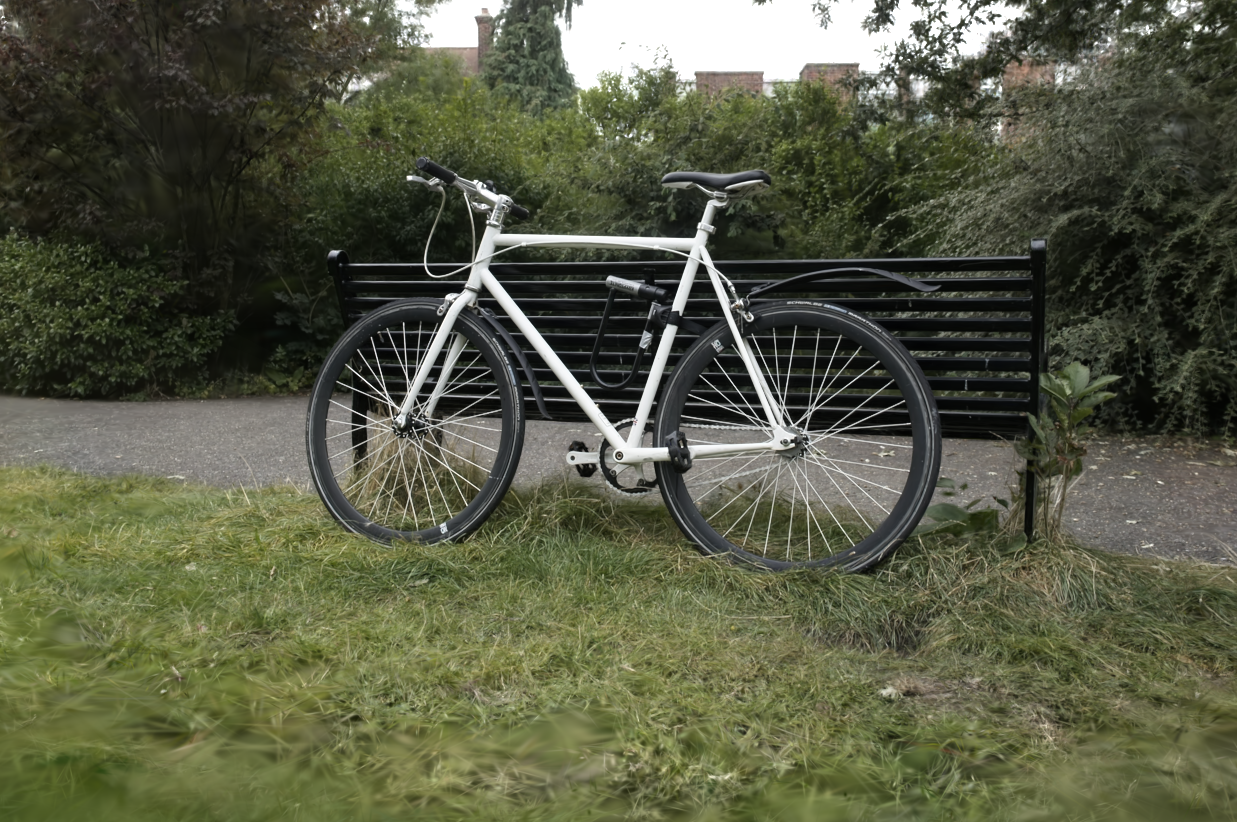
\includegraphics[width=0.3\textwidth]{../o-3dgs/eval/bicycle/test/ours_30000/renders/00000.png} & 
            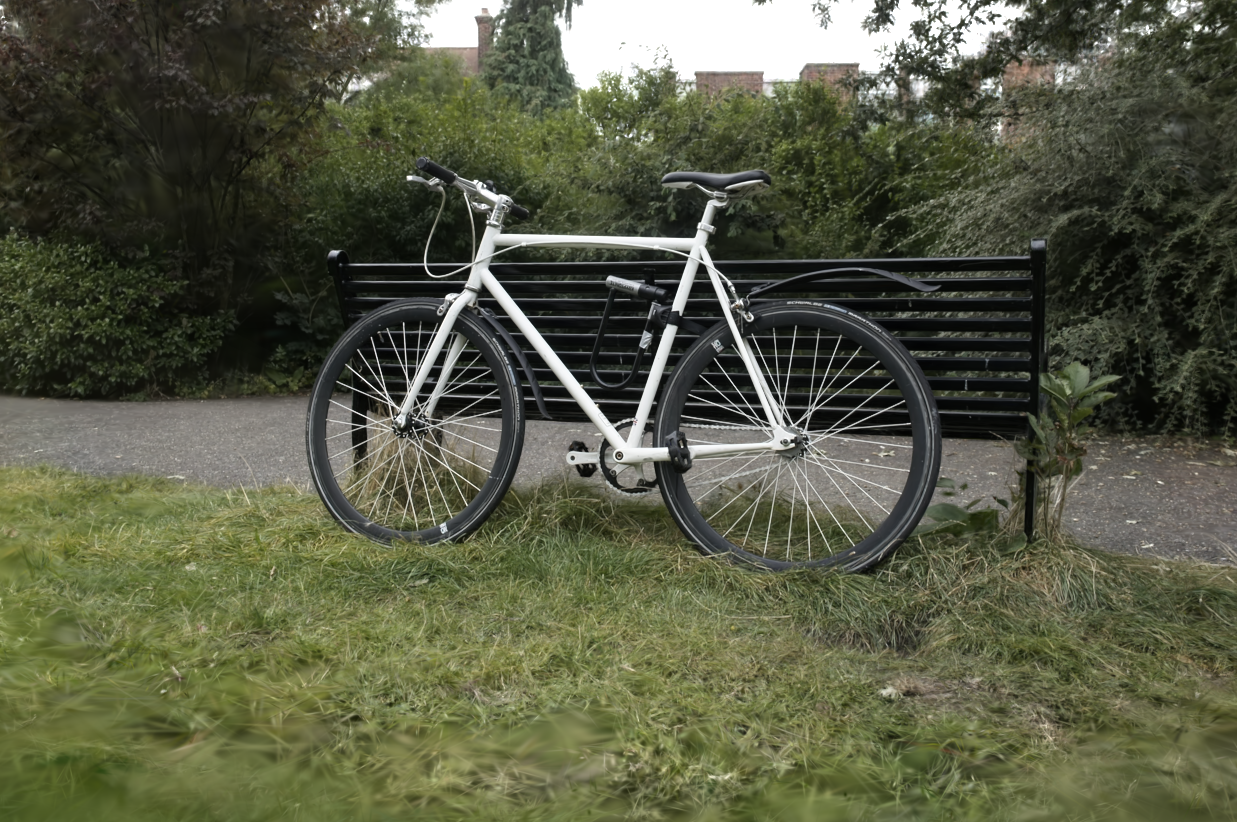
\includegraphics[width=0.3\textwidth]{../o-3dgs/eval/bicycle/test/ours_30000/renders/00000.png} \\
            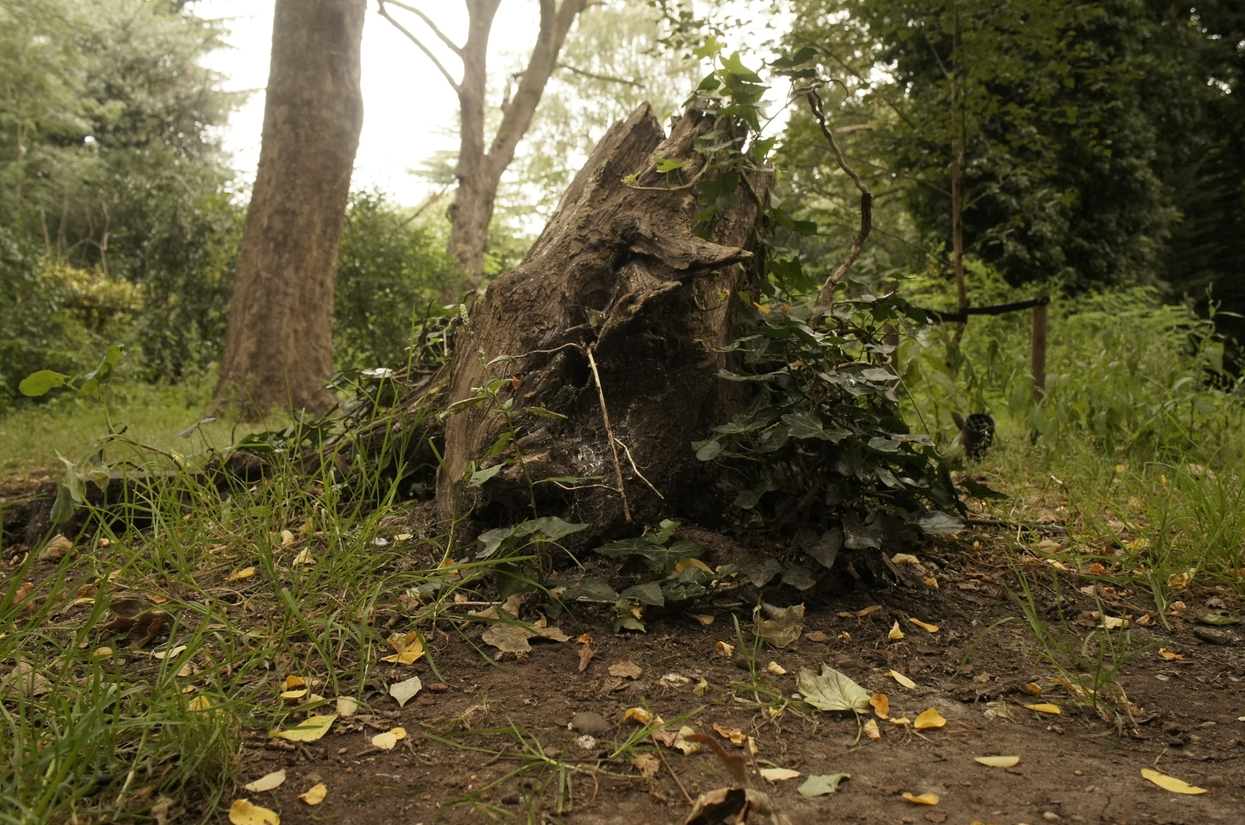
\includegraphics[width=0.3\textwidth]{../o-3dgs/eval/stump/test/ours_30000/gt/00000.png} &
            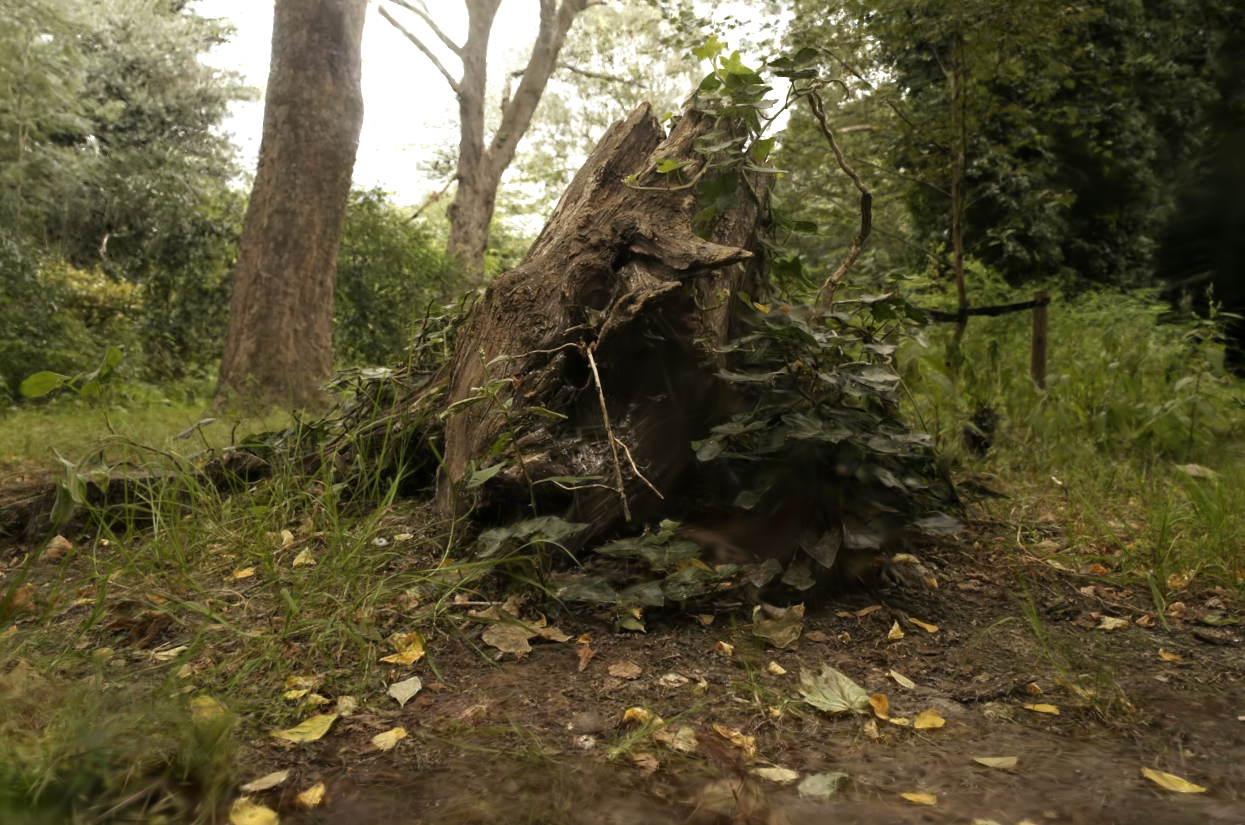
\includegraphics[width=0.3\textwidth]{../o-3dgs/eval/stump/test/ours_30000/renders/00000.png} & 
            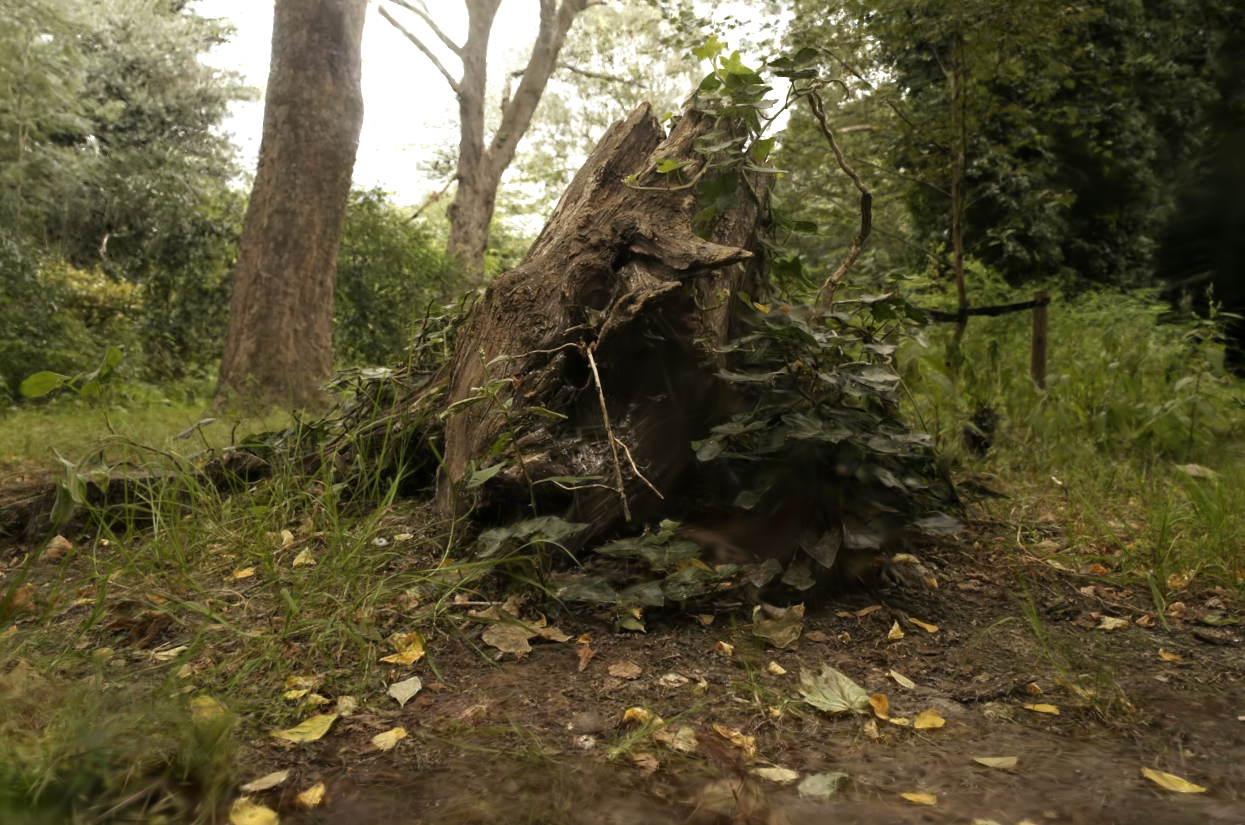
\includegraphics[width=0.3\textwidth]{../o-3dgs/eval/stump/test/ours_30000/renders/00000.png} \\
            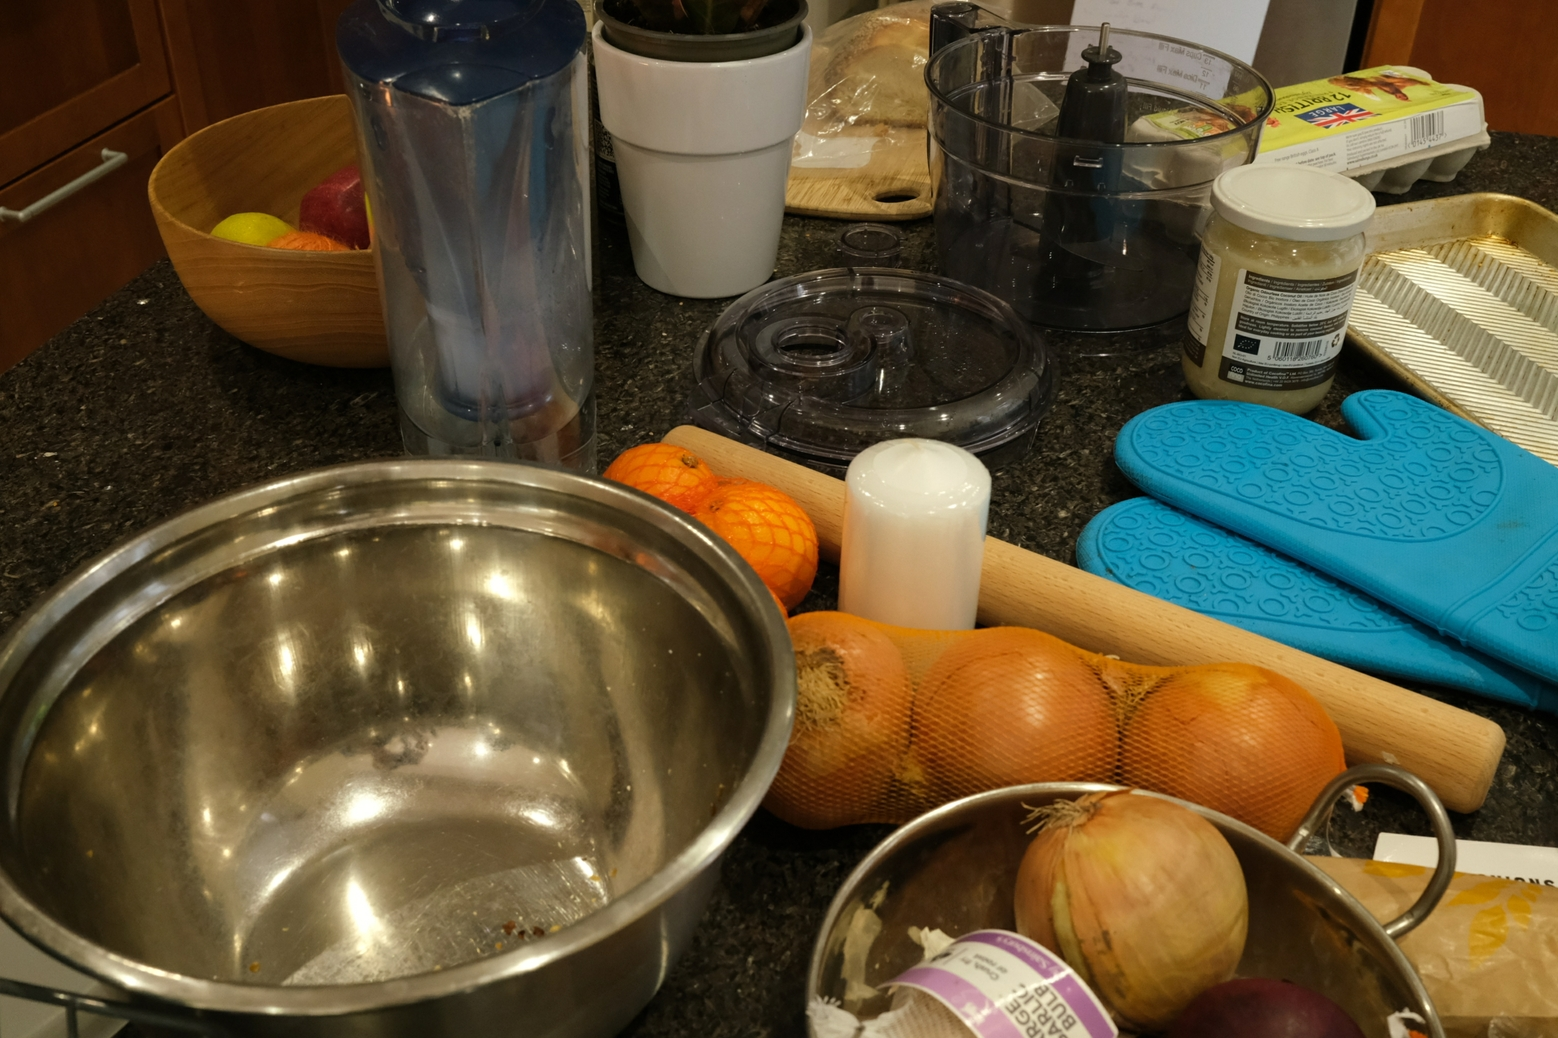
\includegraphics[width=0.3\textwidth]{../o-3dgs/eval/counter/test/ours_30000/gt/00000.png} &
            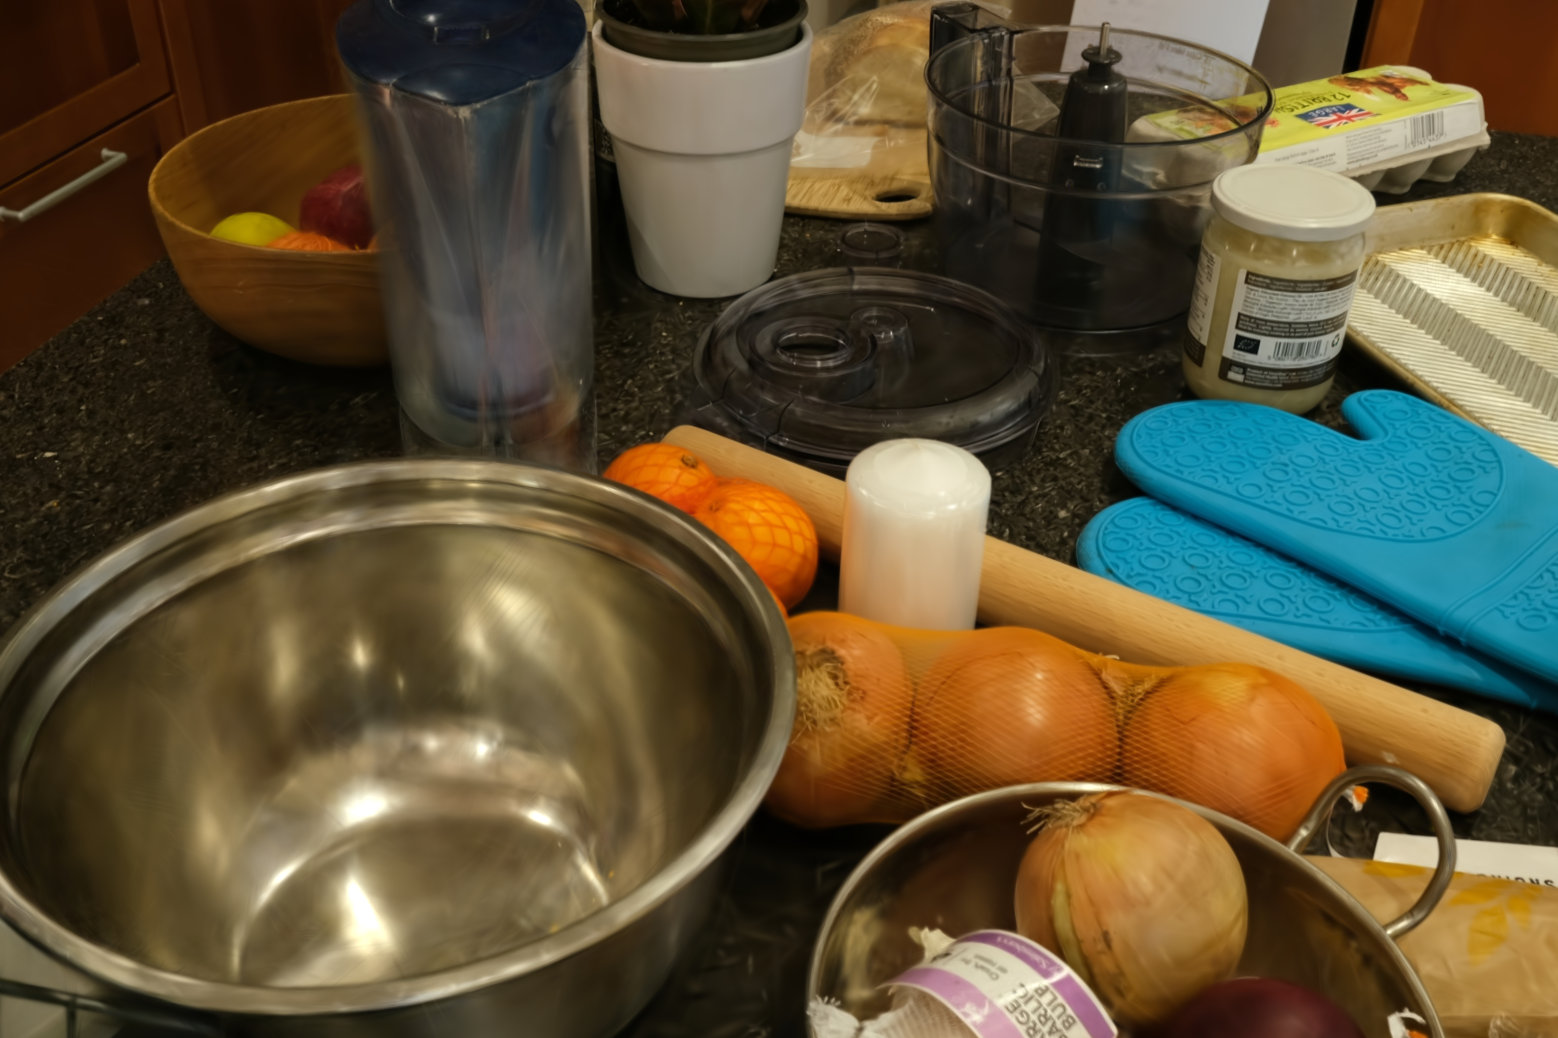
\includegraphics[width=0.3\textwidth]{../o-3dgs/eval/counter/test/ours_30000/renders/00000.png} & 
            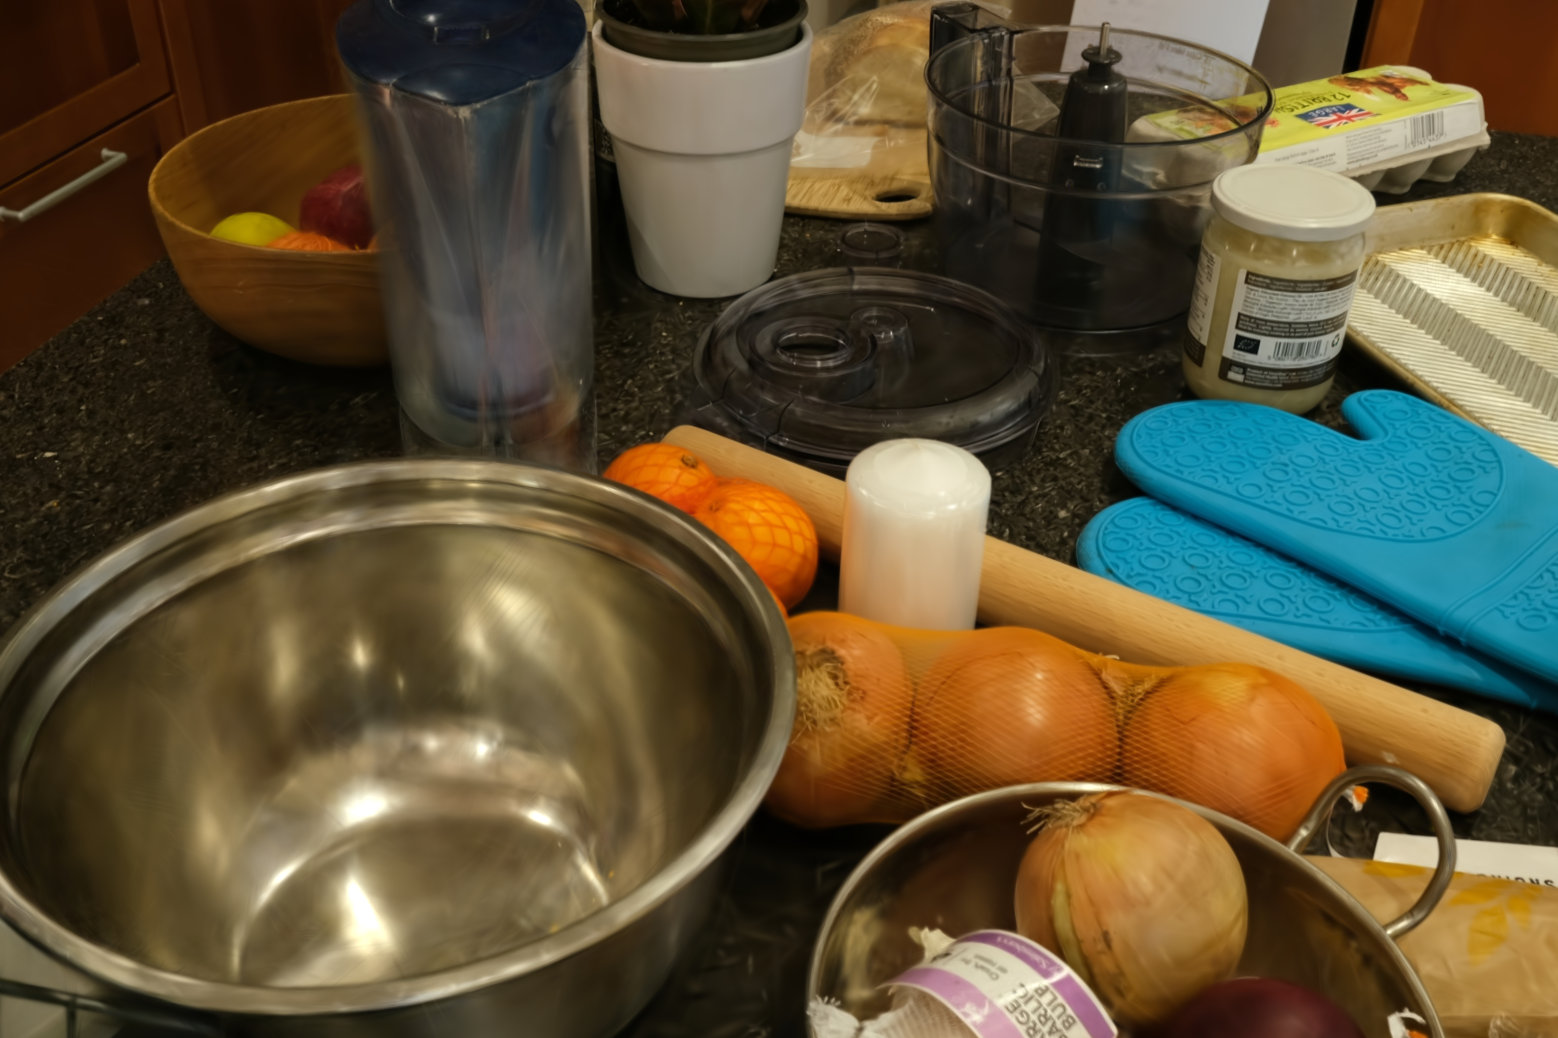
\includegraphics[width=0.3\textwidth]{../o-3dgs/eval/counter/test/ours_30000/renders/00000.png} \\
            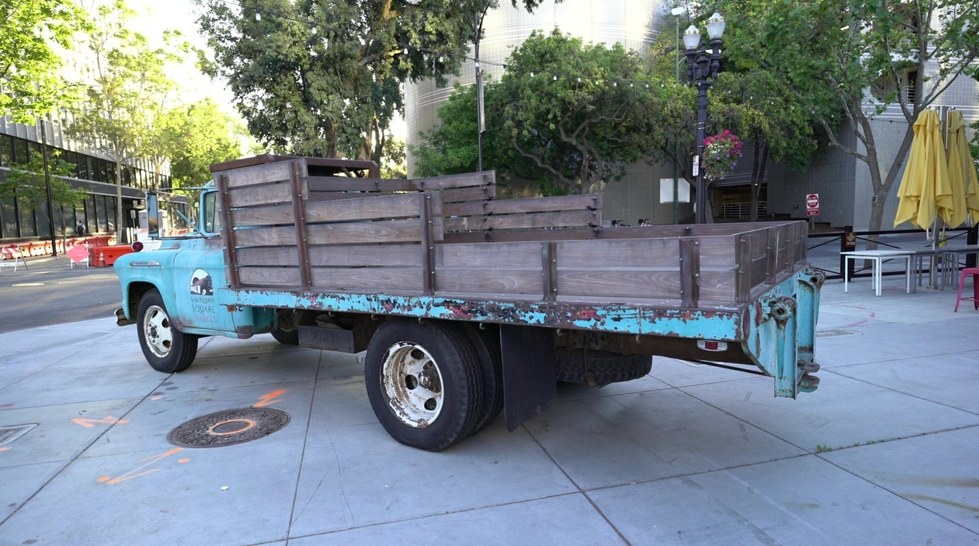
\includegraphics[width=0.3\textwidth]{../o-3dgs/eval/truck/test/ours_30000/gt/00000.png} &
            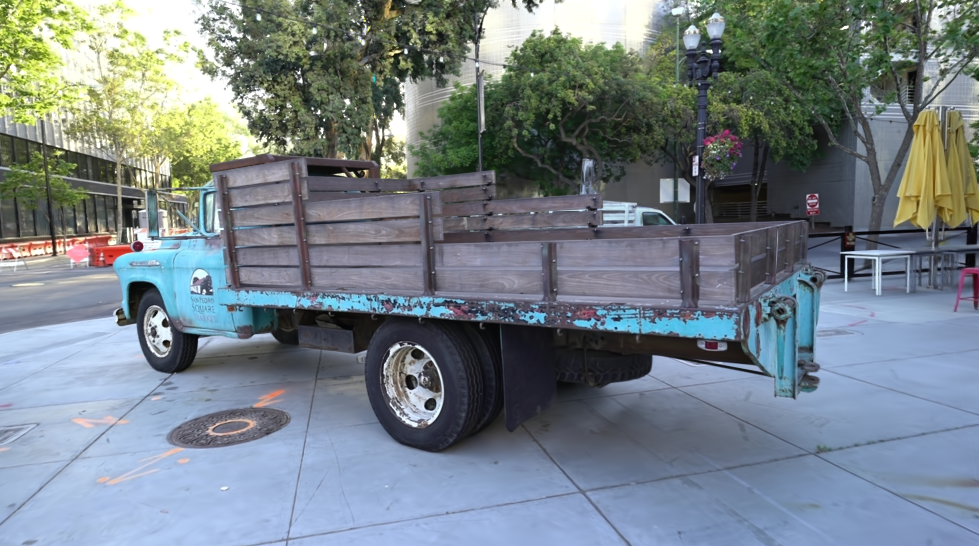
\includegraphics[width=0.3\textwidth]{../o-3dgs/eval/truck/test/ours_30000/renders/00000.png} & 
            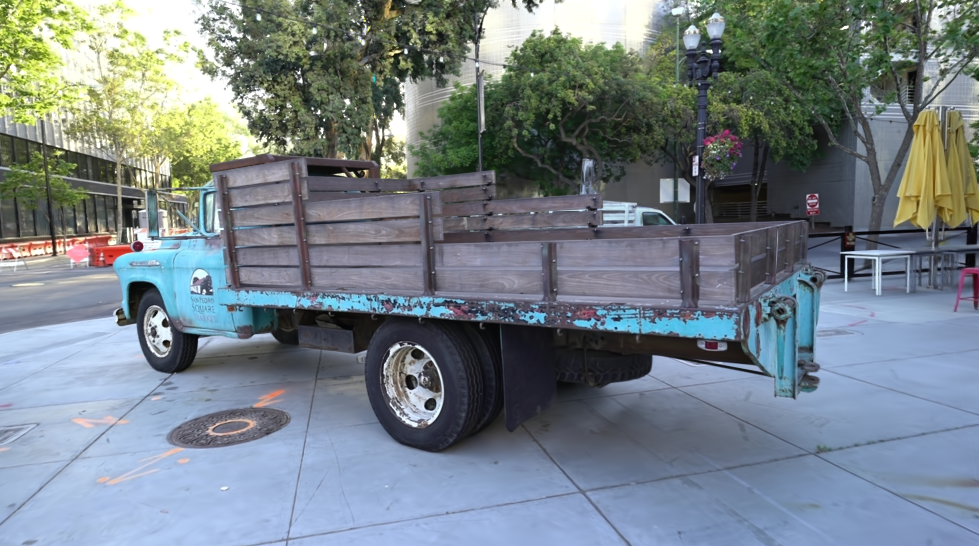
\includegraphics[width=0.3\textwidth]{../o-3dgs/eval/truck/test/ours_30000/renders/00000.png} \\
            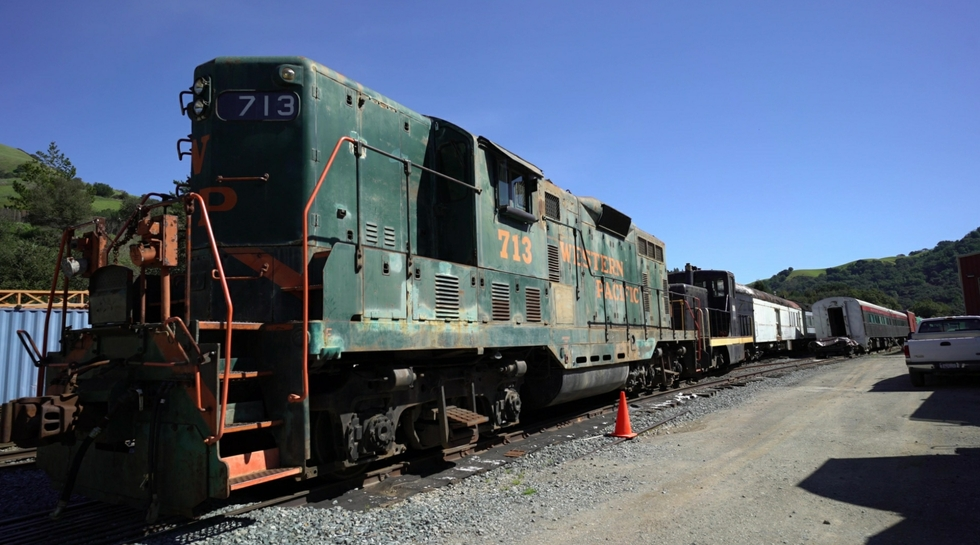
\includegraphics[width=0.3\textwidth]{../o-3dgs/eval/train/test/ours_30000/gt/00000.png} &
            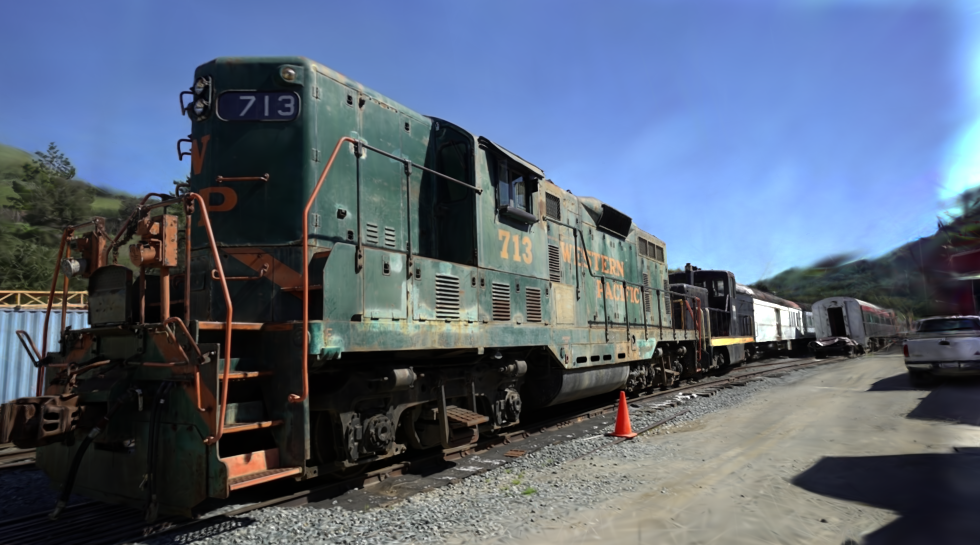
\includegraphics[width=0.3\textwidth]{../o-3dgs/eval/train/test/ours_30000/renders/00000.png} & 
            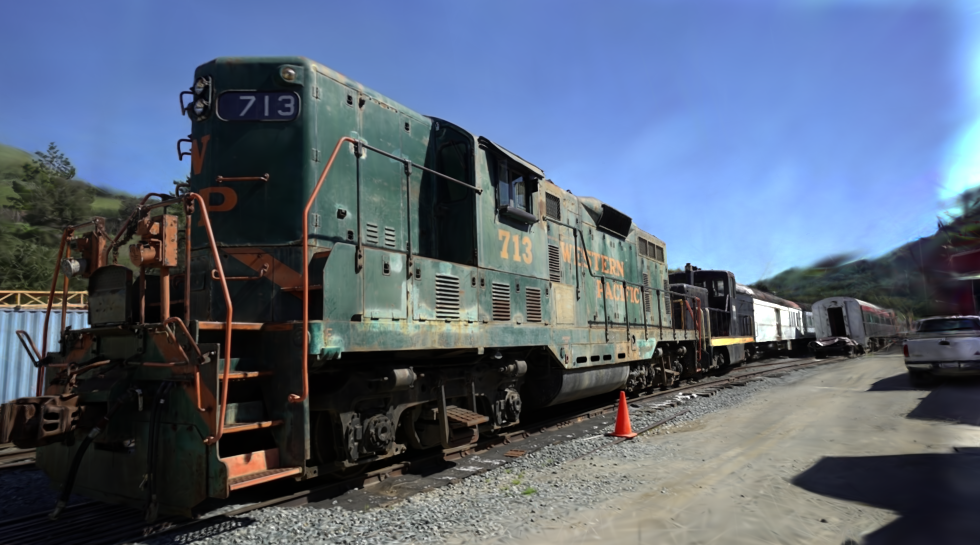
\includegraphics[width=0.3\textwidth]{../o-3dgs/eval/train/test/ours_30000/renders/00000.png} \\
            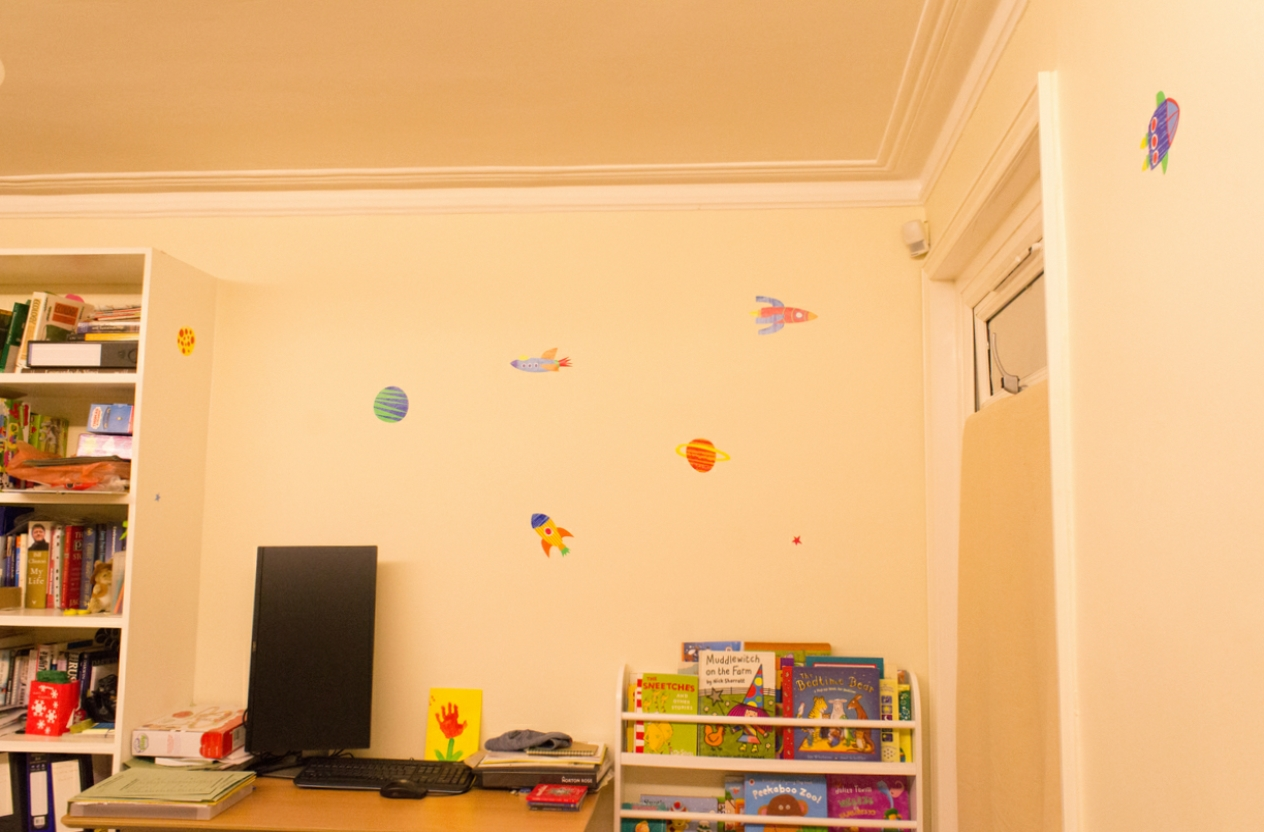
\includegraphics[width=0.3\textwidth]{../o-3dgs/eval/playroom/test/ours_30000/gt/00000.png} &
            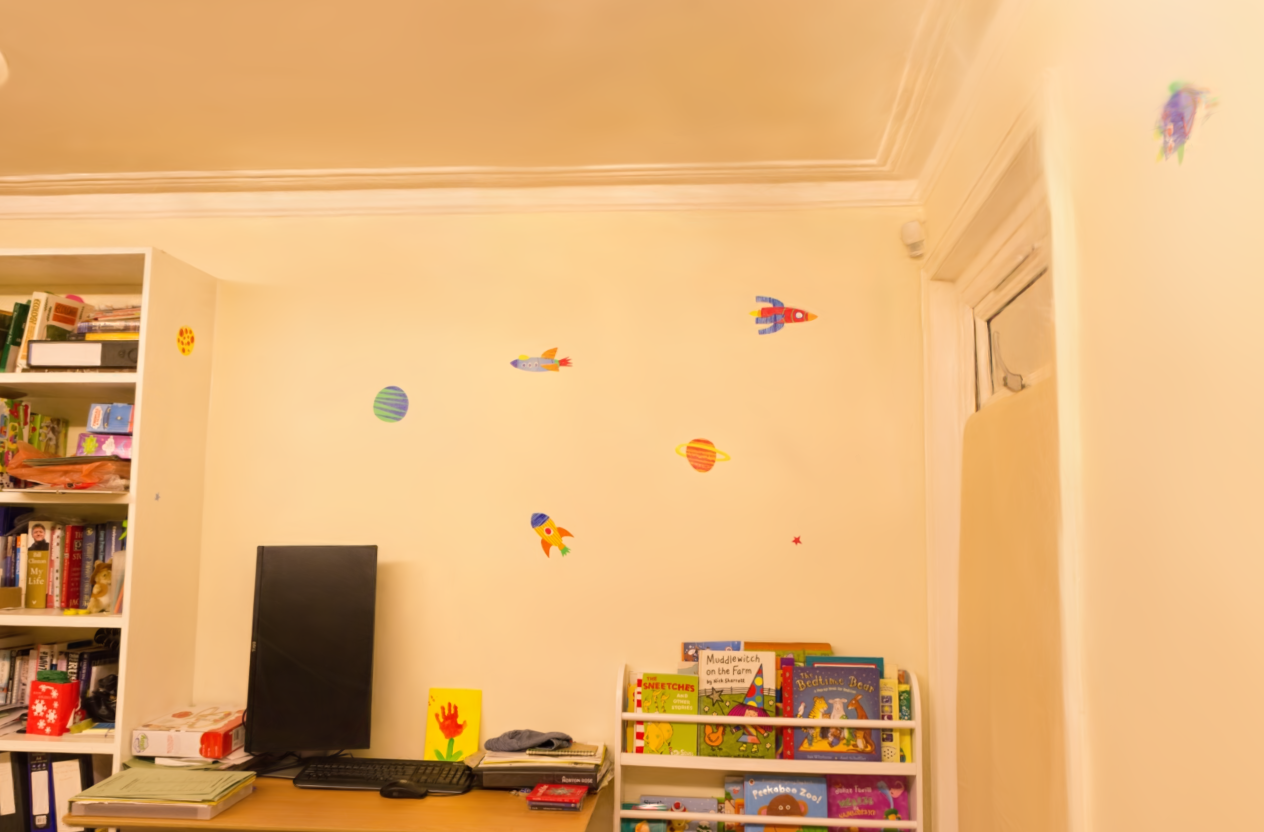
\includegraphics[width=0.3\textwidth]{../o-3dgs/eval/playroom/test/ours_30000/renders/00000.png} & 
            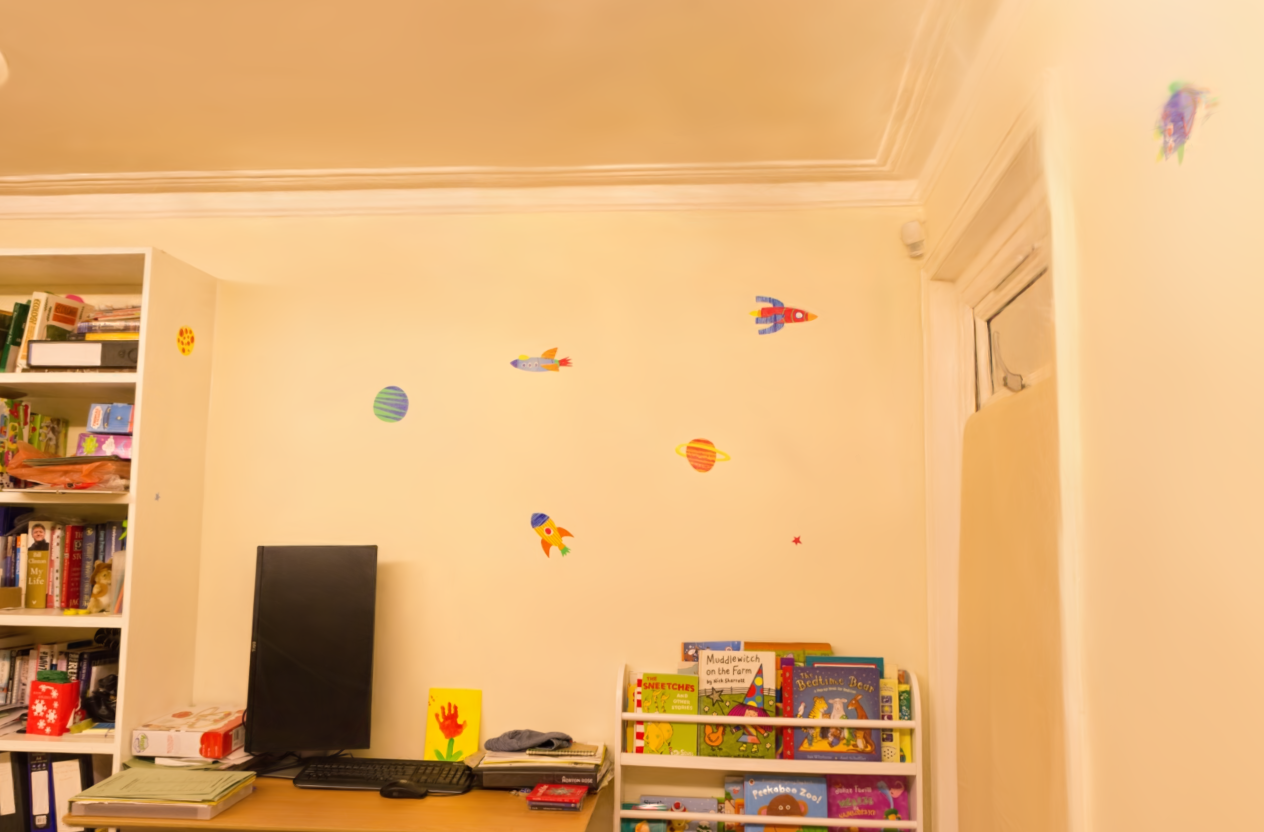
\includegraphics[width=0.3\textwidth]{../o-3dgs/eval/playroom/test/ours_30000/renders/00000.png} \\
            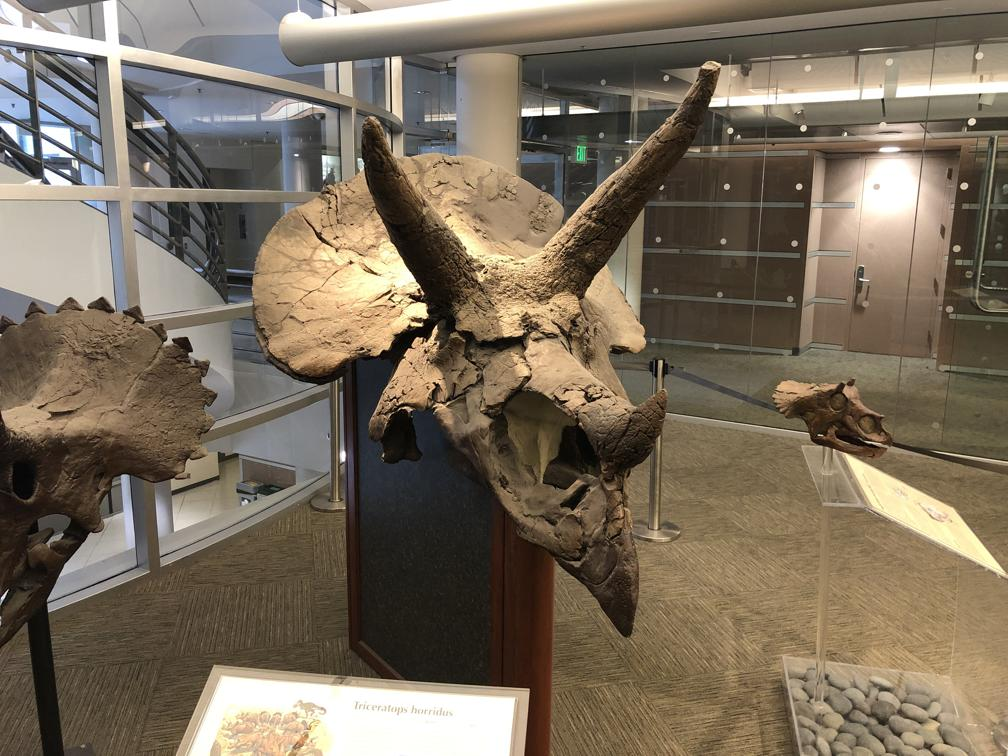
\includegraphics[width=0.3\textwidth]{../o-3dgs/eval/horns/test/ours_30000/gt/00000.png} &
            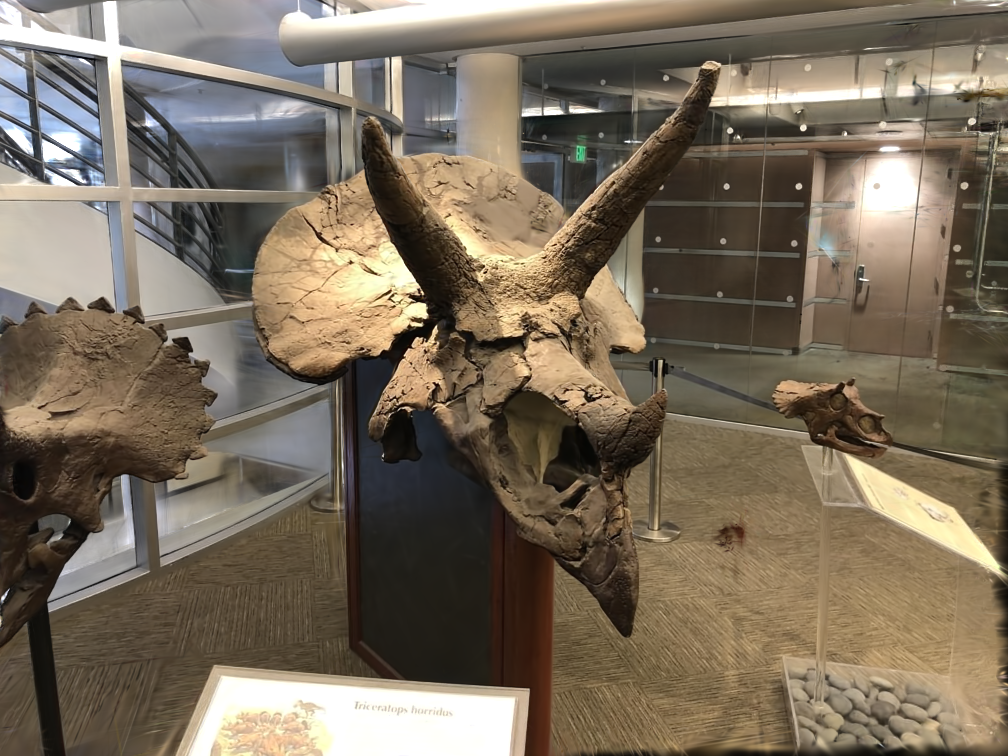
\includegraphics[width=0.3\textwidth]{../o-3dgs/eval/horns/test/ours_30000/renders/00000.png} & 
            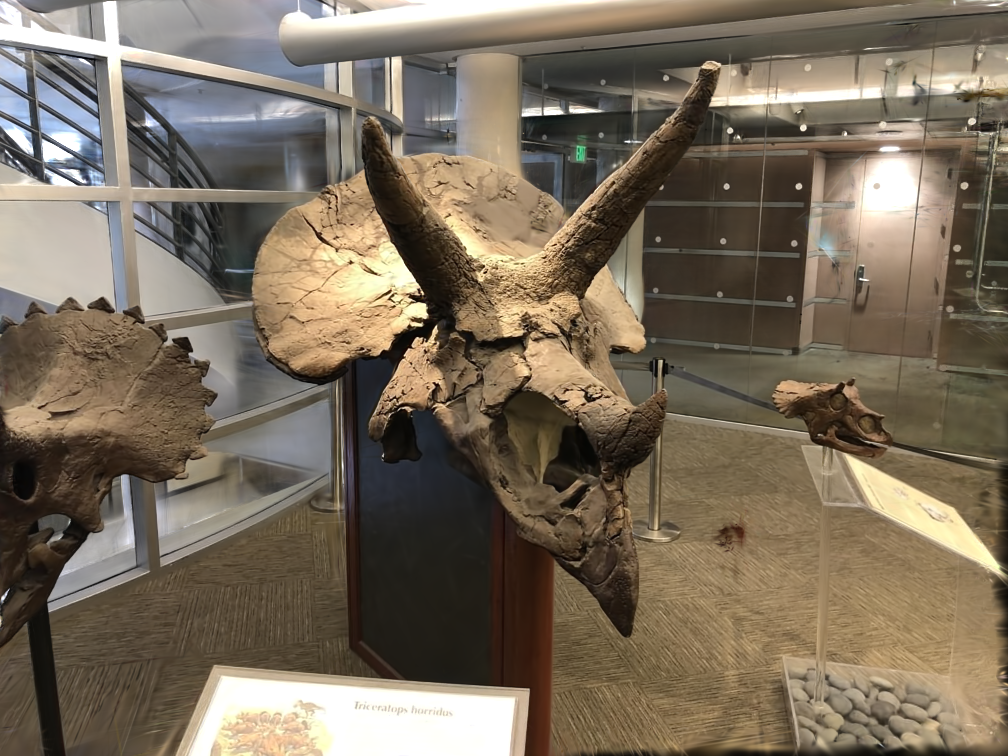
\includegraphics[width=0.3\textwidth]{../o-3dgs/eval/horns/test/ours_30000/renders/00000.png} \\
            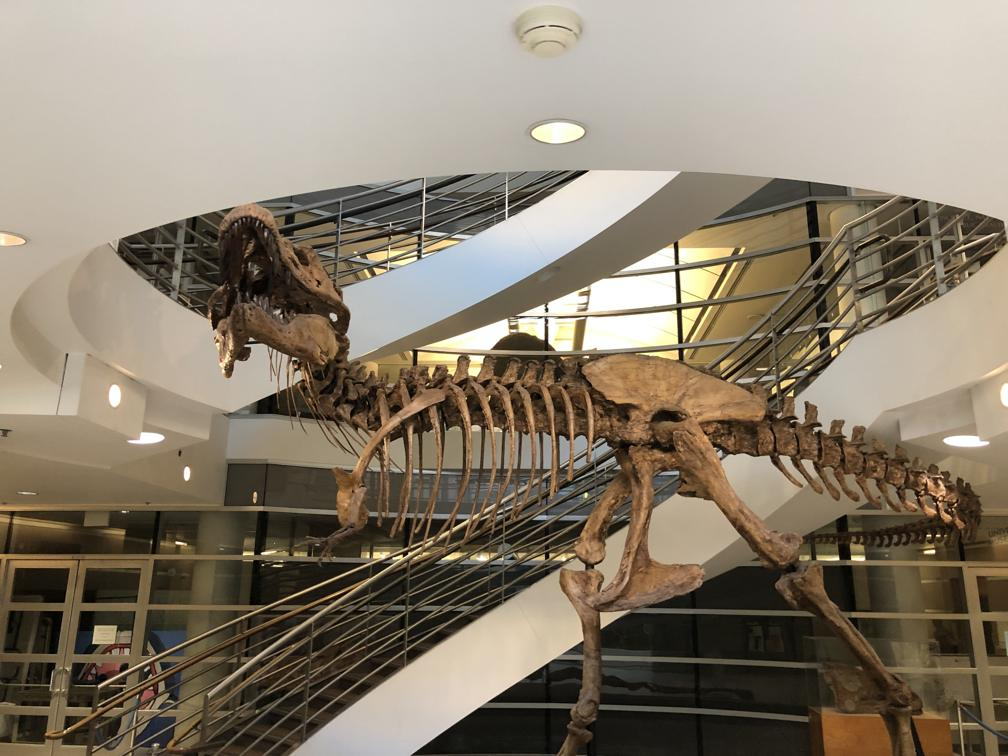
\includegraphics[width=0.3\textwidth]{../o-3dgs/eval/trex/test/ours_30000/gt/00000.png} &
            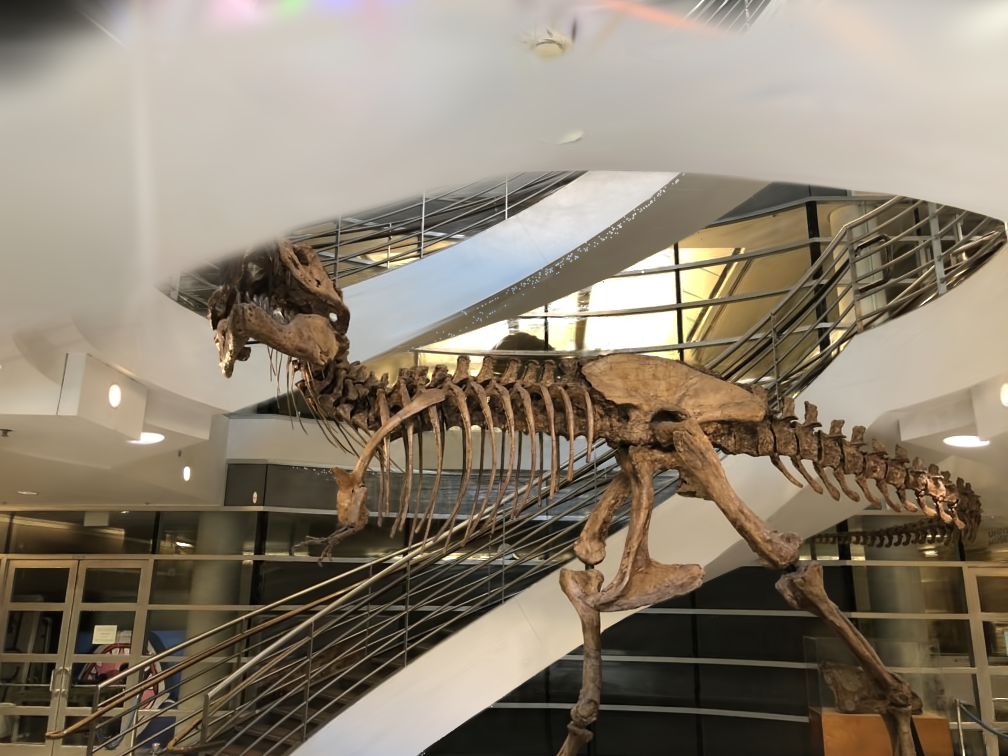
\includegraphics[width=0.3\textwidth]{../o-3dgs/eval/trex/test/ours_30000/renders/00000.png} & 
            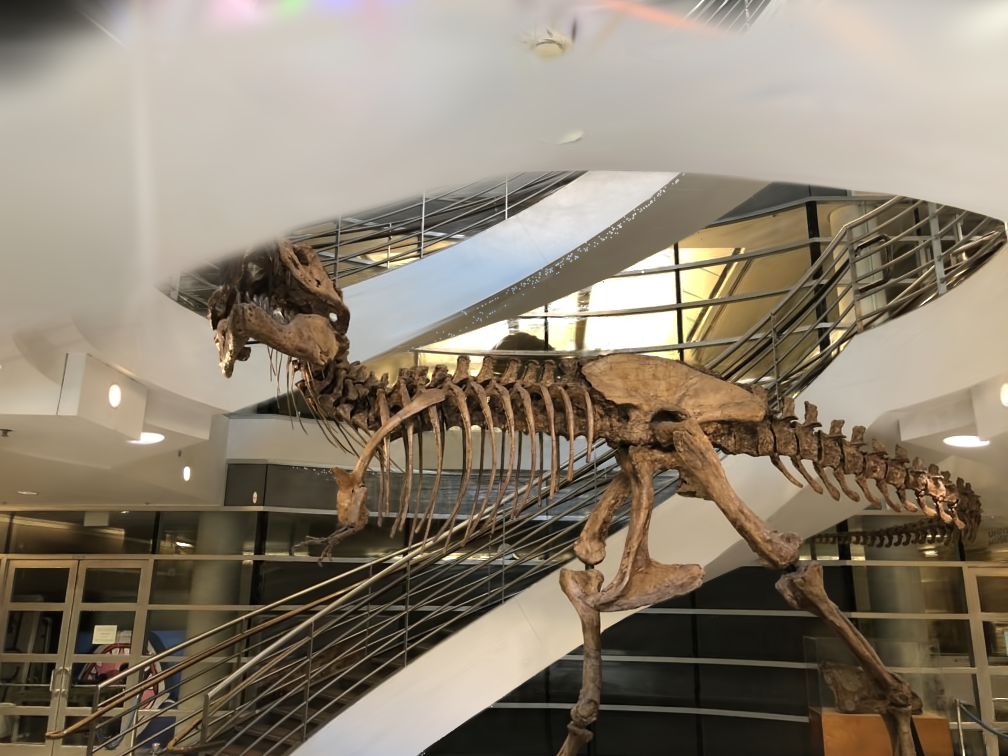
\includegraphics[width=0.3\textwidth]{../o-3dgs/eval/trex/test/ours_30000/renders/00000.png} \\
    \end{tabular}
    

    \begin{tabular}{llccccc}
    \toprule
    \textbf{Category} & \textbf{Scene} & \textbf{Method} & \textbf{SSIM$\uparrow$} & \textbf{PSNR$\uparrow$} & \textbf{LPIPS$\downarrow$} & \textbf{Mem} \\
    \midrule
    \multirow{8}{*}{\textbf{MipNeRF360 Indoor}} & 
        \multirow{2}{*}{Counter} 
        & 3D-GS & 0.909 & 29.10 & 0.199 & 255MB \\
            & & \textbf{Our Model} & 0.909 & 29.07 & \textbf{0.198} & 275MB \\
            \cmidrule{2-7} &
        \multirow{2}{*}{Kitchen} 
        & 3D-GS & 0.928 & 31.49 & 0.125 & 378MB \\
            & & \textbf{Our Model} & 0.928 & 31.40 & 0.126 & 393MB \\
            \cmidrule{2-7} &
        \multirow{2}{*}{Bonsai} 
        & 3D-GS & 0.943 & 32.34 & 0.204 & 252MB \\
            & & \textbf{Our Model} & 0.942 & \textbf{32.35} & \textbf{0.203} & 263MB \\
            \cmidrule{2-7} &
        \multirow{2}{*}{Room} 
        & 3D-GS & 0.921 & 31.65 & 0.217 & 309MB \\
            & & \textbf{Our Model} & 0.920 & \textbf{31.66} & \textbf{0.215} & 340MB \\
        \midrule
    \multirow{2}{*}{\textbf{Tanks \& Temples}} & 
        \multirow{2}{*}{Train} 
        & 3D-GS & 0.821 & 22.13 & 0.196 & 257MB \\
            & & \textbf{Our Model} & 0.821 & \textbf{22.19} & 0.197 & 273MB \\
        \midrule
    \multirow{4}{*}{\textbf{LLFF}} & 
        \multirow{2}{*}{Horns} 
        & 3D-GS & 0.887 & 27.21 & 0.132 & 157MB \\
            & & \textbf{Our Model} & 0.887 & \textbf{27.32} & 0.134 & 163MB \\
            \cmidrule{2-7} &
        \multirow{2}{*}{Trex} 
        & 3D-GS & 0.899 & 25.59 & 0.130 & 110MB \\
            & & \textbf{Our Model} & \textbf{0.909} & \textbf{26.66} & \textbf{0.116} & 116MB \\
    \bottomrule
    \end{tabular}

\chapter{Conclusions and Future Directions}

\section{Conclusions}
In this project, we explored the use of 3D Gaussian Splatting for real-time radiance field rendering. We introduced an adaptive density control mechanism to dynamically adjust the number of Gaussians in the scene, leading to improved representation and rendering quality. Our results demonstrate the effectiveness of this approach in various scenes.

\section{Discussion of Limitations}
While our method shows significant improvements, it has some limitations. The adaptive density control mechanism can be computationally expensive, and the choice of parameters such as the threshold $\epsilon_\alpha$ can significantly impact the results. Additionally, our method may struggle with extremely complex scenes where the number of Gaussians required becomes prohibitively large.

\section{Future Directions}
Future research could focus on optimizing the adaptive density control mechanism to reduce computational overhead. Exploring alternative representations and hybrid approaches could further enhance the scalability and efficiency of the method. Additionally, investigating the integration of our approach with other neural rendering techniques could lead to even more robust and versatile solutions.

\end{document}